\documentclass[11pt,a4paper]{article}

\usepackage[utf8]{inputenc}
\usepackage[T1]{fontenc}
\usepackage[brazil]{babel}
\usepackage{geometry}
\geometry{
  a4paper,
  top=2.5cm,
  bottom=2.5cm,
  left=2.5cm,
  right=2.5cm
}

\usepackage{amsmath,amssymb,amsfonts,amsthm}
\usepackage{graphicx}
\usepackage{booktabs}
\usepackage{tabularx}
\usepackage{multirow}
\usepackage{xcolor}
\usepackage{hyperref}
\usepackage{float}
\usepackage{caption}
\usepackage{subcaption}
\usepackage{microtype}
\usepackage{enumitem}
\usepackage{cite}

\hypersetup{
    colorlinks=true,
    linkcolor=blue!70!black,
    citecolor=blue!70!black,
    urlcolor=blue!70!black
}

\title{\textbf{Projeto Finor -- Index Tracking do S\&P 100 e do Ibovespa:\\
Modelagem Quantitativa, Estrutura de Mercado e Controle de Turnover}}
\author{\textbf{Pedro de Paula Odorize}\\[0.5em]
\textit{Bootcamp de Data Science Finor 2026}}
\date{Outubro de 2026}

\begin{document}

\maketitle

\begin{abstract}
Este trabalho apresenta o desenvolvimento, a análise exploratória e a validação empírica de um modelo quantitativo de \textit{Index Tracking} (rastreamento passivo de índices) com restrição estrita de cardinalidade ($K \le 10$) e penalidade de giro (\textit{turnover}) para o \textbf{S\&P 100} (mercado acionário dos EUA) e o \textbf{IBOVESPA} (mercado brasileiro), cobrindo sete anos de histórico (2019 a 2026). A partir de uma rigorosa auditoria em mais de 302 mil retornos diários que corrigiu distorções de bases públicas, formulamos o problema como uma Programação Quadrática Inteira Mista (MIQP) e traçamos a Fronteira de Pareto (\textit{Tracking Error} vs. Giro) em 20 trimestres consecutivos fora da amostra (\textit{walk-forward}). Demonstramos teoricamente e empiricamente a decomposição euclidiana entre RMSE, Tracking Error e Viés via Teorema de Pitágoras no $\mathbb{R}^T$. Os resultados revelam que a incorporação da penalidade de giro na função objetivo atua como um regularizador estrutural: no Ibovespa, calibrar $\lambda_{\text{anual}} = 3.0$ reduziu o Tracking Error fora da amostra de 4,50\% para 4,37\% ao ano e reduziu o giro trimestral em 74\% (de 21,5\% para 5,56\%), com custos de transação explícitos (15 bps na B3 e 5 bps nos EUA). No teste de hipótese contra um modelo nulo de Monte Carlo com 1.000 carteiras aleatórias, o modelo ótimo superou 100\% das carteiras no S\&P 100 ($p < 0,001$) e 99\% no Ibovespa ($p = 0,01$).
\end{abstract}

\vspace{1em}
\noindent\textbf{Palavras-chave:} Index Tracking, MIQP, Tracking Error, Turnover Constraint, Fronteira de Pareto, Ibovespa, S\&P 100, Finanças Quantitativas.

\newpage
\tableofcontents
\newpage

% ==============================================================================
\section{Resumo Executivo}
% ==============================================================================

O projeto tem como objetivo central construir carteiras passivas concentradas em poucas ações ($K = 5, 10, 20$) que acompanhem com máxima fidelidade o retorno diário de dois benchmarks de naturezas distintas: o \textbf{S\&P 100} (índice de preços das 100 maiores empresas americanas) e o \textbf{Ibovespa} (índice de retorno total com as ações mais líquidas do Brasil).

\subsection*{Principais Descobertas com os Dados}
\begin{enumerate}[leftmargin=*]
    \item \textbf{Dados auditados com incerteza declarada:} Identificamos e corrigimos um problema grave de código reaproveitado na Natura (\texttt{NATU3}) e dois erros de proventos do Yahoo Finance na Ultrapar (\texttt{UGPA3}) e na Copasa (\texttt{CSMG3}), confrontando-os com os boletins oficiais da B3 (COTAHIST). Dos 460 retornos diários extremos ($\ge \pm 15\%$), decompusemos 186 como reflexo de choque de mercado e 272 como eventos idiossincráticos da empresa ou setor. Uma auditoria amostral em 50 desses eventos comprovou 100\% de veracidade.
    \item \textbf{Nenhum ativo isolado replica o índice:} A ação mais correlacionada explica no máximo 65\% da variância ($R^2 \le 0,65$; a maior correlação foi de \texttt{ITSA4} com 0,81 no Ibov). Isso comprova a necessidade mandatória de modelos de otimização combinatória.
    \item \textbf{Descolamento do S\&P 100 pós-2023:} Desde 2023, a correlação média entre as ações americanas despencou de 0,43 para 0,19 devido ao rali altamente concentrado em poucas gigantes de tecnologia (\textit{Magnificent Seven}). Pela Análise de Componentes Principais (PCA), são necessários 41 fatores para explicar 80\% da variância recente do S\&P 100, contra 30 no Ibovespa.
    \item \textbf{Assimetria de Cauda no Brasil:} No Ibovespa, as ações caem em bloco durante momentos de estresse (correlação mediana de 0,64 nos 10\% piores dias), mas sobem de forma dispersa (0,43 nos 10\% melhores dias), refletindo a prevalência do risco soberano/fiscal em períodos de crise.
\end{enumerate}

\subsection*{O que a Modelagem Revelou}
\begin{enumerate}[leftmargin=*]
    \item \textbf{Desempenho com 10 ações:} O Tracking Error (TE) fora da amostra estabiliza-se em 4,91\% a.a. no S\&P 100 e 4,52\% a.a. no Ibovespa, com $R^2 > 0,92$.
    \item \textbf{Otimização vs. Heurística Ingênua:} Selecionar as 10 ações mais correlacionadas e alocar pesos resulta em erros quase duas vezes maiores (8,25\% no S\&P e 9,95\% no Ibov), pois essa abordagem negligencia a covariância e sobrecarrega um único setor.
    \item \textbf{O Efeito Regularizador da Penalidade de Giro:} A incorporação da penalidade de turnover no MIQP permitiu derrubar o giro trimestral no Ibovespa de 21,5\% para 5,56\% e no S\&P 100 de 26,4\% para 4,52\%, aumentando a rentabilidade líquida de custos de transação e reduzindo o Tracking Error fora da amostra.
\end{enumerate}

% ==============================================================================
\section{Formulação Matemática e Métricas de Erro}
% ==============================================================================

\subsection{O Problema de Index Tracking (MIQP)}
Seja $R_t$ o retorno do benchmark no pregão $t$, $r_{t,i}$ o retorno da ação $i \in I$ e $w_i$ o peso alocado. O problema com restrição de cardinalidade $K$ e penalidade de giro $\lambda_{\text{anual}}$ é formulado como:

\begin{equation}
\min_{w, z, s} \; \underbrace{252 \cdot \left[ \frac{1}{T} \sum_{t=1}^T \left( R_t - \sum_{i \in I} w_i r_{t,i} \right)^2 \right]}_{\approx \text{TE}^2 \text{ anual de calibração}} + \lambda_{\text{anual}} \cdot \underbrace{\left( 4 \sum_{j \in S_{\text{prev}}} s_j + 4 w_{\text{deslistadas}} \right)}_{\text{Turnover anualizado}}
\label{eq:miqp_obj}
\end{equation}

\noindent sujeito a:
\begin{align}
\sum_{i \in I} w_i &= 1 \quad &\text{(Orçamento 100\% investido)} \label{eq:budget}\\
0 \le w_i &\le z_i \quad \forall i \in I \quad &\text{(Posições long-only)} \label{eq:coupling}\\
\sum_{i \in I} z_i &\le K \quad &\text{(Cardinalidade máxima de } K \text{ ações)} \label{eq:cardinality}\\
s_j &\ge w_j^{\text{drift}} - w_j, \quad s_j \ge 0 \quad \forall j \in S_{\text{prev}} \quad &\text{(Volume de vendas da carteira prévia)} \label{eq:turnover_slack}\\
z_i &\in \{0, 1\} \quad \forall i \in I \label{eq:binary}
\end{align}

\noindent onde $w_j^{\text{drift}}$ é o peso do ativo $j$ ao final do trimestre de teste anterior após derivar com a oscilação dos preços.

\subsection{A Relação Euclidiana entre RMSE, Tracking Error e Viés}
Seja o erro diário $e_t = r_{\text{carteira}, t} - R_{\text{índice}, t}$, com média amostral $\bar{e} = \frac{1}{T}\sum e_t$. Pela decomposição de variância:
\begin{equation}
\text{MSE}_{\text{diário}} = \frac{1}{T}\sum_{t=1}^T e_t^2 = s_e^2 + \bar{e}^2
\end{equation}

Em termos de anualização em finanças:
\begin{itemize}
    \item O \textbf{Tracking Error (TE)} escala com a raiz do tempo: $\text{TE} = s_e \sqrt{252} \implies s_e^2 = \frac{\text{TE}^2}{252}$.
    \item O \textbf{Viés (drift)} escala linearmente: $\text{Viés} = 252 \cdot \bar{e} \implies \bar{e}^2 = \frac{\text{Viés}^2}{252^2}$.
    \item O \textbf{RMSE anualizado} segue a escala de volatilidade: $\text{RMSE}^2 = 252 \cdot \text{MSE}_{\text{diário}}$.
\end{itemize}

Multiplicando a equação por 252, obtemos a identidade exata:
\begin{equation}
\mathbf{\text{RMSE}_{\text{anual}}^2 = \text{TE}^2 + \frac{\text{Viés}^2}{252}}
\label{eq:pitagoras}
\end{equation}

\noindent Geometricamente, no espaço $\mathbb{R}^T$, o vetor de erros $\mathbf{e}$ decompõe-se ortogonalmente em um vetor paralelo à média $\bar{e}\mathbf{1}$ (o viés) e um vetor residual centrado $\mathbf{e} - \bar{e}\mathbf{1}$ (o tracking error). O Teorema de Pitágoras garante a igualdade. Como o viés anual ($\sim 2\%$) dividido por 252 gera um termo de ordem $10^{-4}$, a hipotenusa ($\text{RMSE}$) é numericamente indistinguível do cateto ($\text{TE}$) até a segunda casa decimal.

% ==============================================================================
\section{Coleta e Higienização dos Dados}
% ==============================================================================

\subsection{Convenções de Preços e Calendários}
\begin{itemize}
    \item \textbf{S\&P 100 (^OEX):} Índice de retorno de preços (\textit{price return}, não reinveste proventos). Para manter perfeita coerência, utilizamos as cotações de fechamento bruto (\texttt{Close}) para os componentes.
    \item \textbf{IBOVESPA (^BVSP):} Índice de retorno total (\textit{total return}, reinveste dividendos e JCP). Utilizamos cotações de fechamento ajustado (\texttt{Adj Close}) da B3.
\end{itemize}

\subsection{Correções Críticas Realizadas}
\begin{enumerate}
    \item \textbf{Natura (\texttt{NATU3}):} A re-listagem da companhia em 02/07/2025 reaproveitou o código antigo encerrado em 2019. Ligar as séries criava uma queda artificial de 72\%. A série foi recortada para manter unicamente o trecho a partir de julho/2025.
    \item \textbf{Ultrapar (\texttt{UGPA3}):} Em 28/06/2021, o Yahoo registrava salto de R\$ 8,75 para R\$ 19,19 (+119\%). A cotação oficial da B3 provou que a cotação real foi de R\$ 18,99 para R\$ 19,19 (+1,05\%). A base histórica anterior do Yahoo estava descalibrada por um fator de 2,2x.
    \item \textbf{Copasa (\texttt{CSMG3}):} Em 19/11/2020, o Yahoo antecipou o desconto do dividendo extraordinário de R\$ 6,49 em um pregão, gerando oscilações falsas de +16,9\% e -12,4\%. A série foi alinhada com as datas-ex oficiais da B3.
\end{enumerate}

\begin{figure}[H]
    \centering
    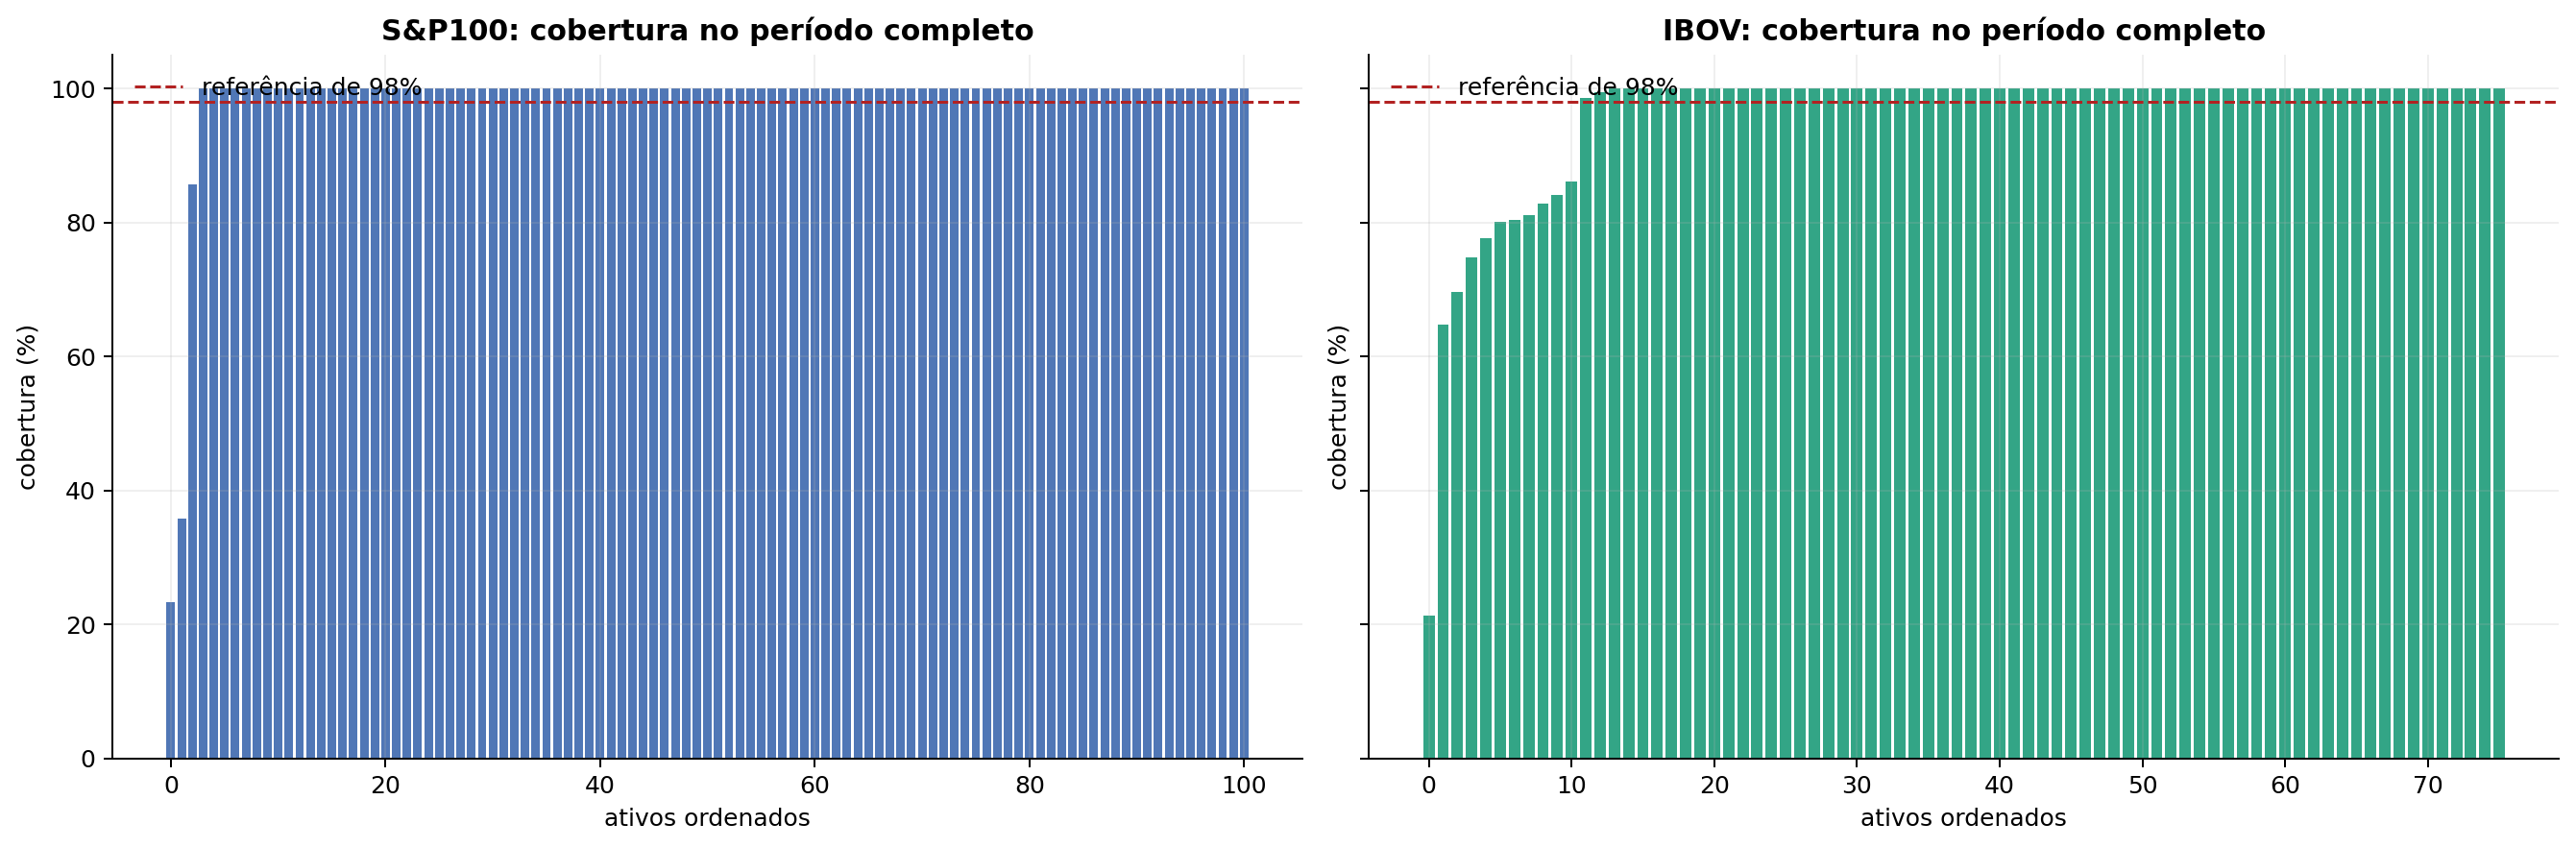
\includegraphics[width=0.85\textwidth]{figures/01_cobertura_dados.png}
    \caption{Completude histórica das ações dos universos S\&P 100 e Ibovespa ao longo dos 7 anos.}
    \label{fig:cobertura}
\end{figure}

% ==============================================================================
\section{Estrutura de Mercado e Descobertas Empíricas}
% ==============================================================================

\subsection{Distribuição de Retornos e Caudas Gordas}
As séries diárias de retornos dos índices apresentam curtose elevada (13,1 no S\&P 100 e 20,7 no Ibovespa), muito acima de uma distribuição normal teórica (curtose = 0). Ocorrências com variações além de $\pm 5\%$ foram 13 no S\&P e 16 no Ibovespa, concentradas no crash da COVID-19 (março/2020).

\begin{figure}[H]
    \centering
    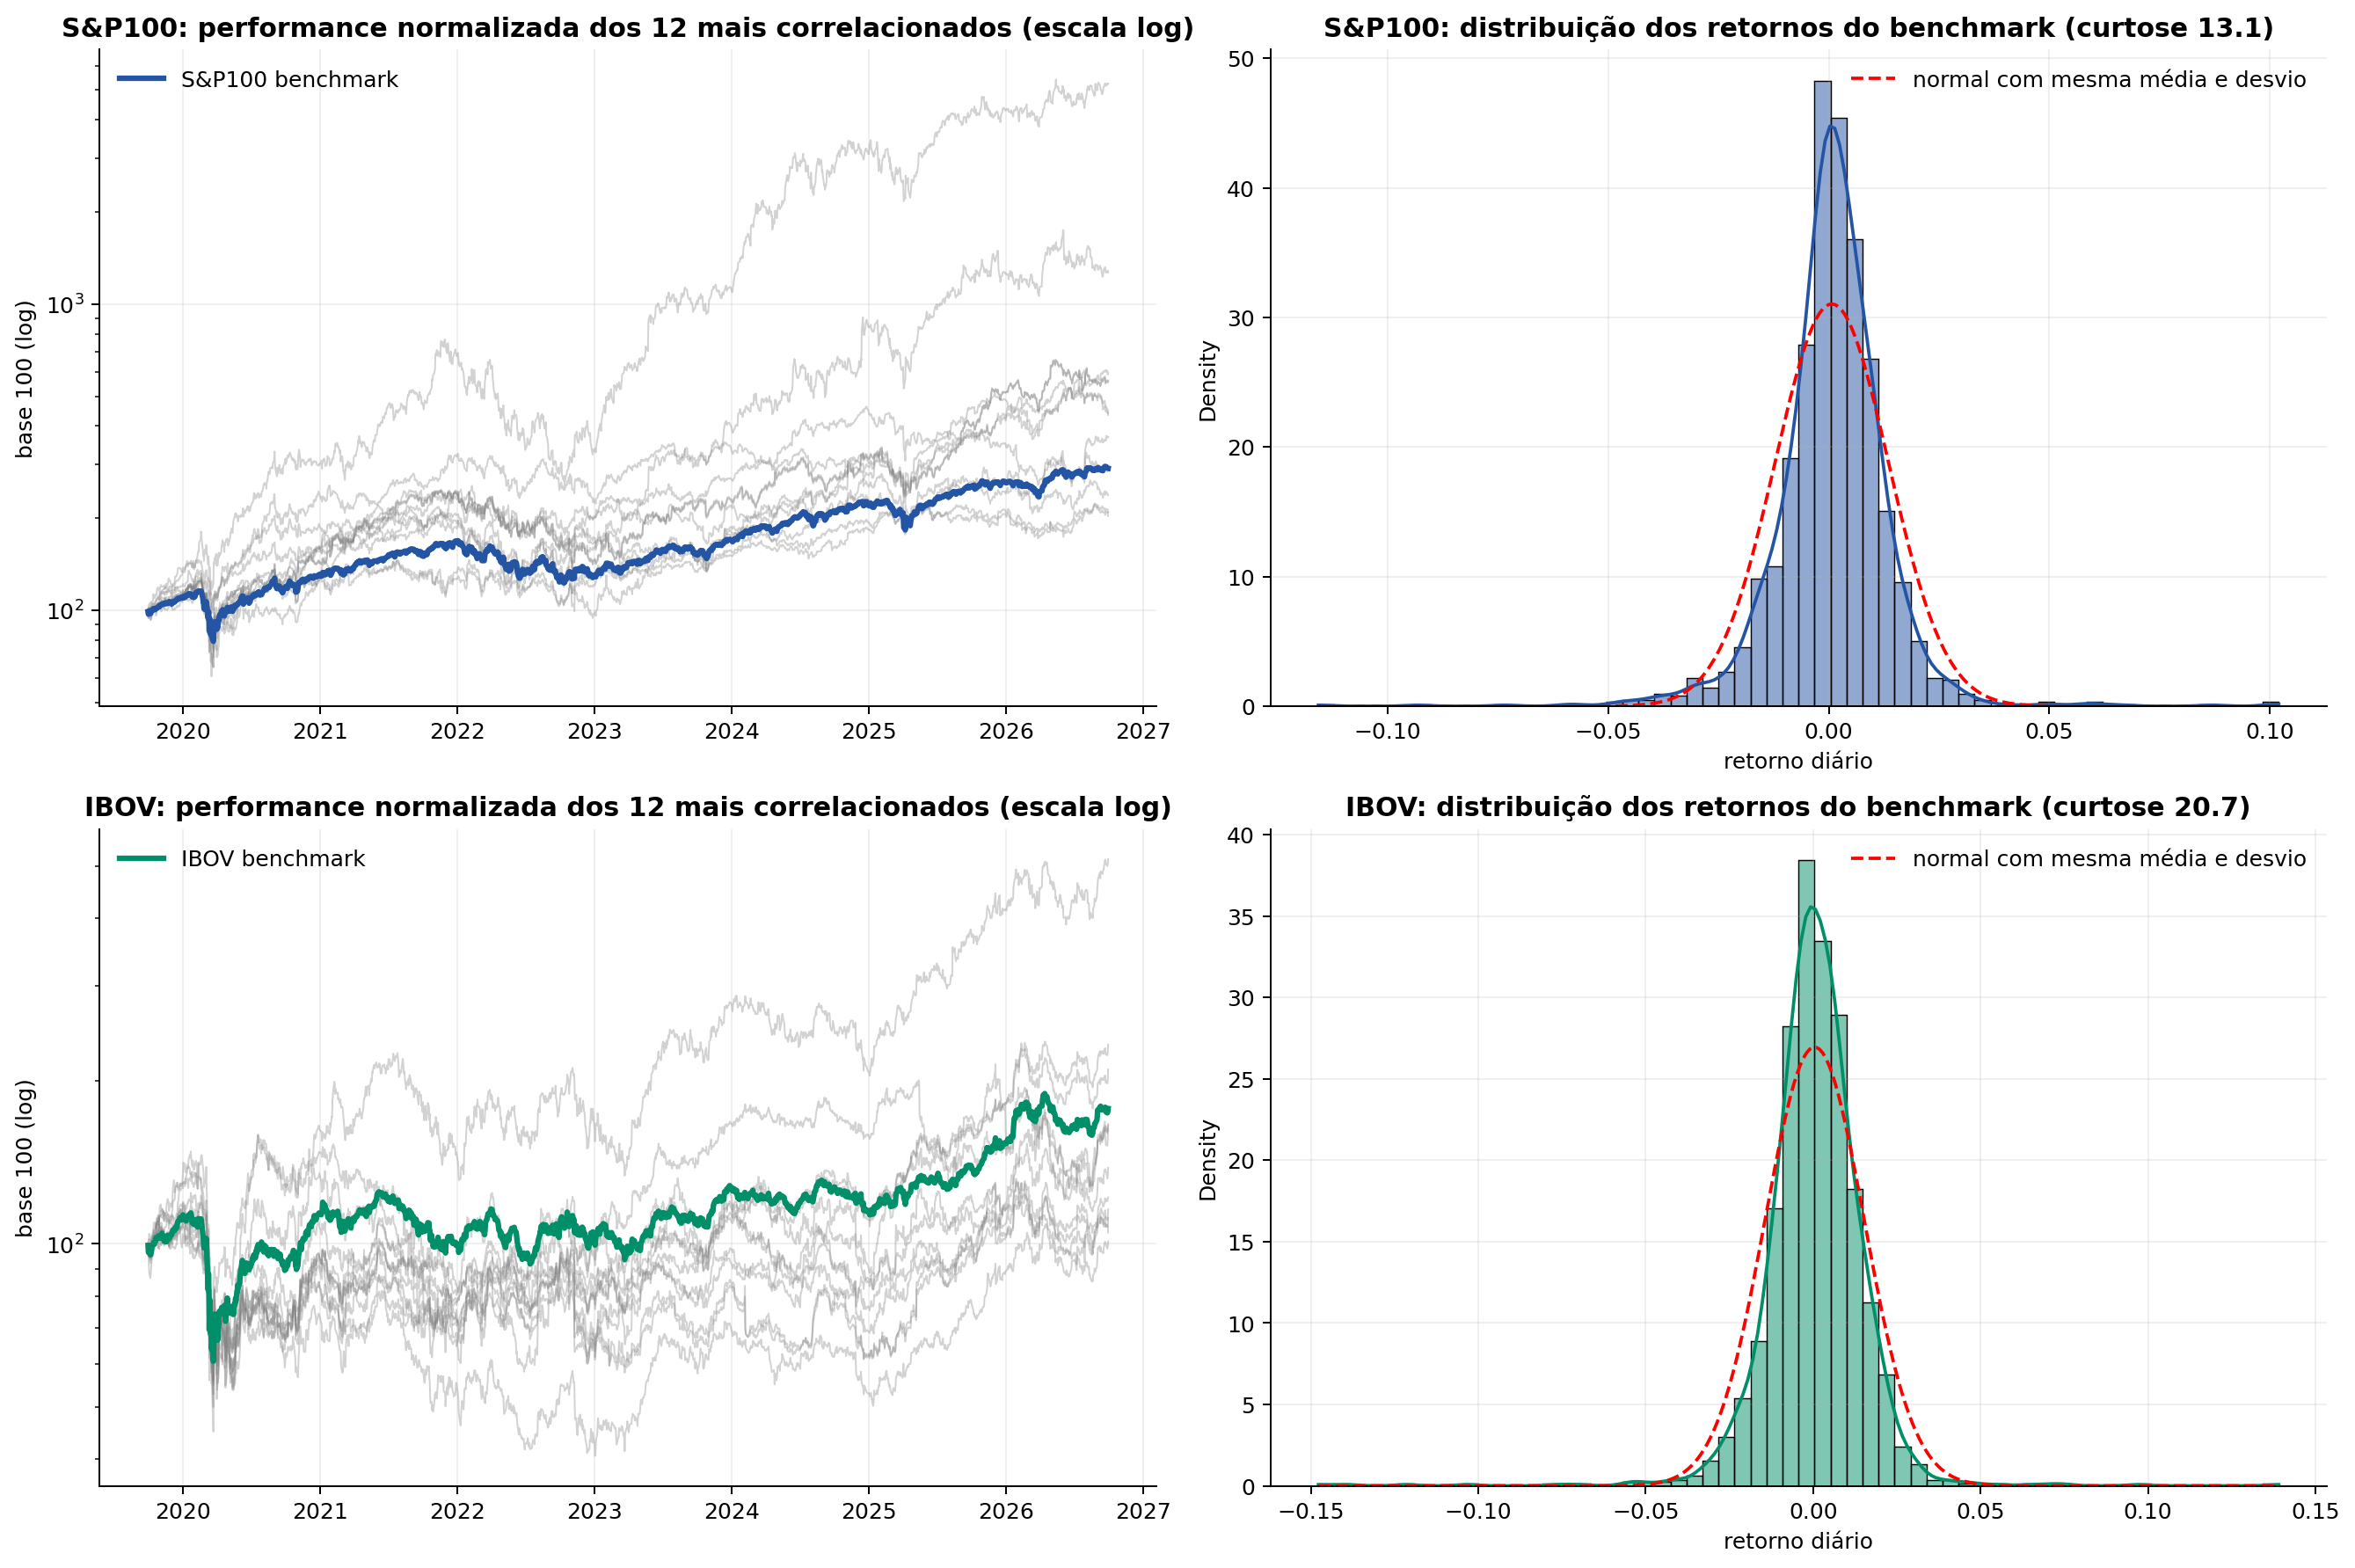
\includegraphics[width=0.9\textwidth]{figures/02_performance_distribuicoes.png}
    \caption{Evolução normalizada (base 100) e distribuição dos retornos diários frente à curva normal teórica.}
    \label{fig:performance_dist}
\end{figure}

\begin{figure}[H]
    \centering
    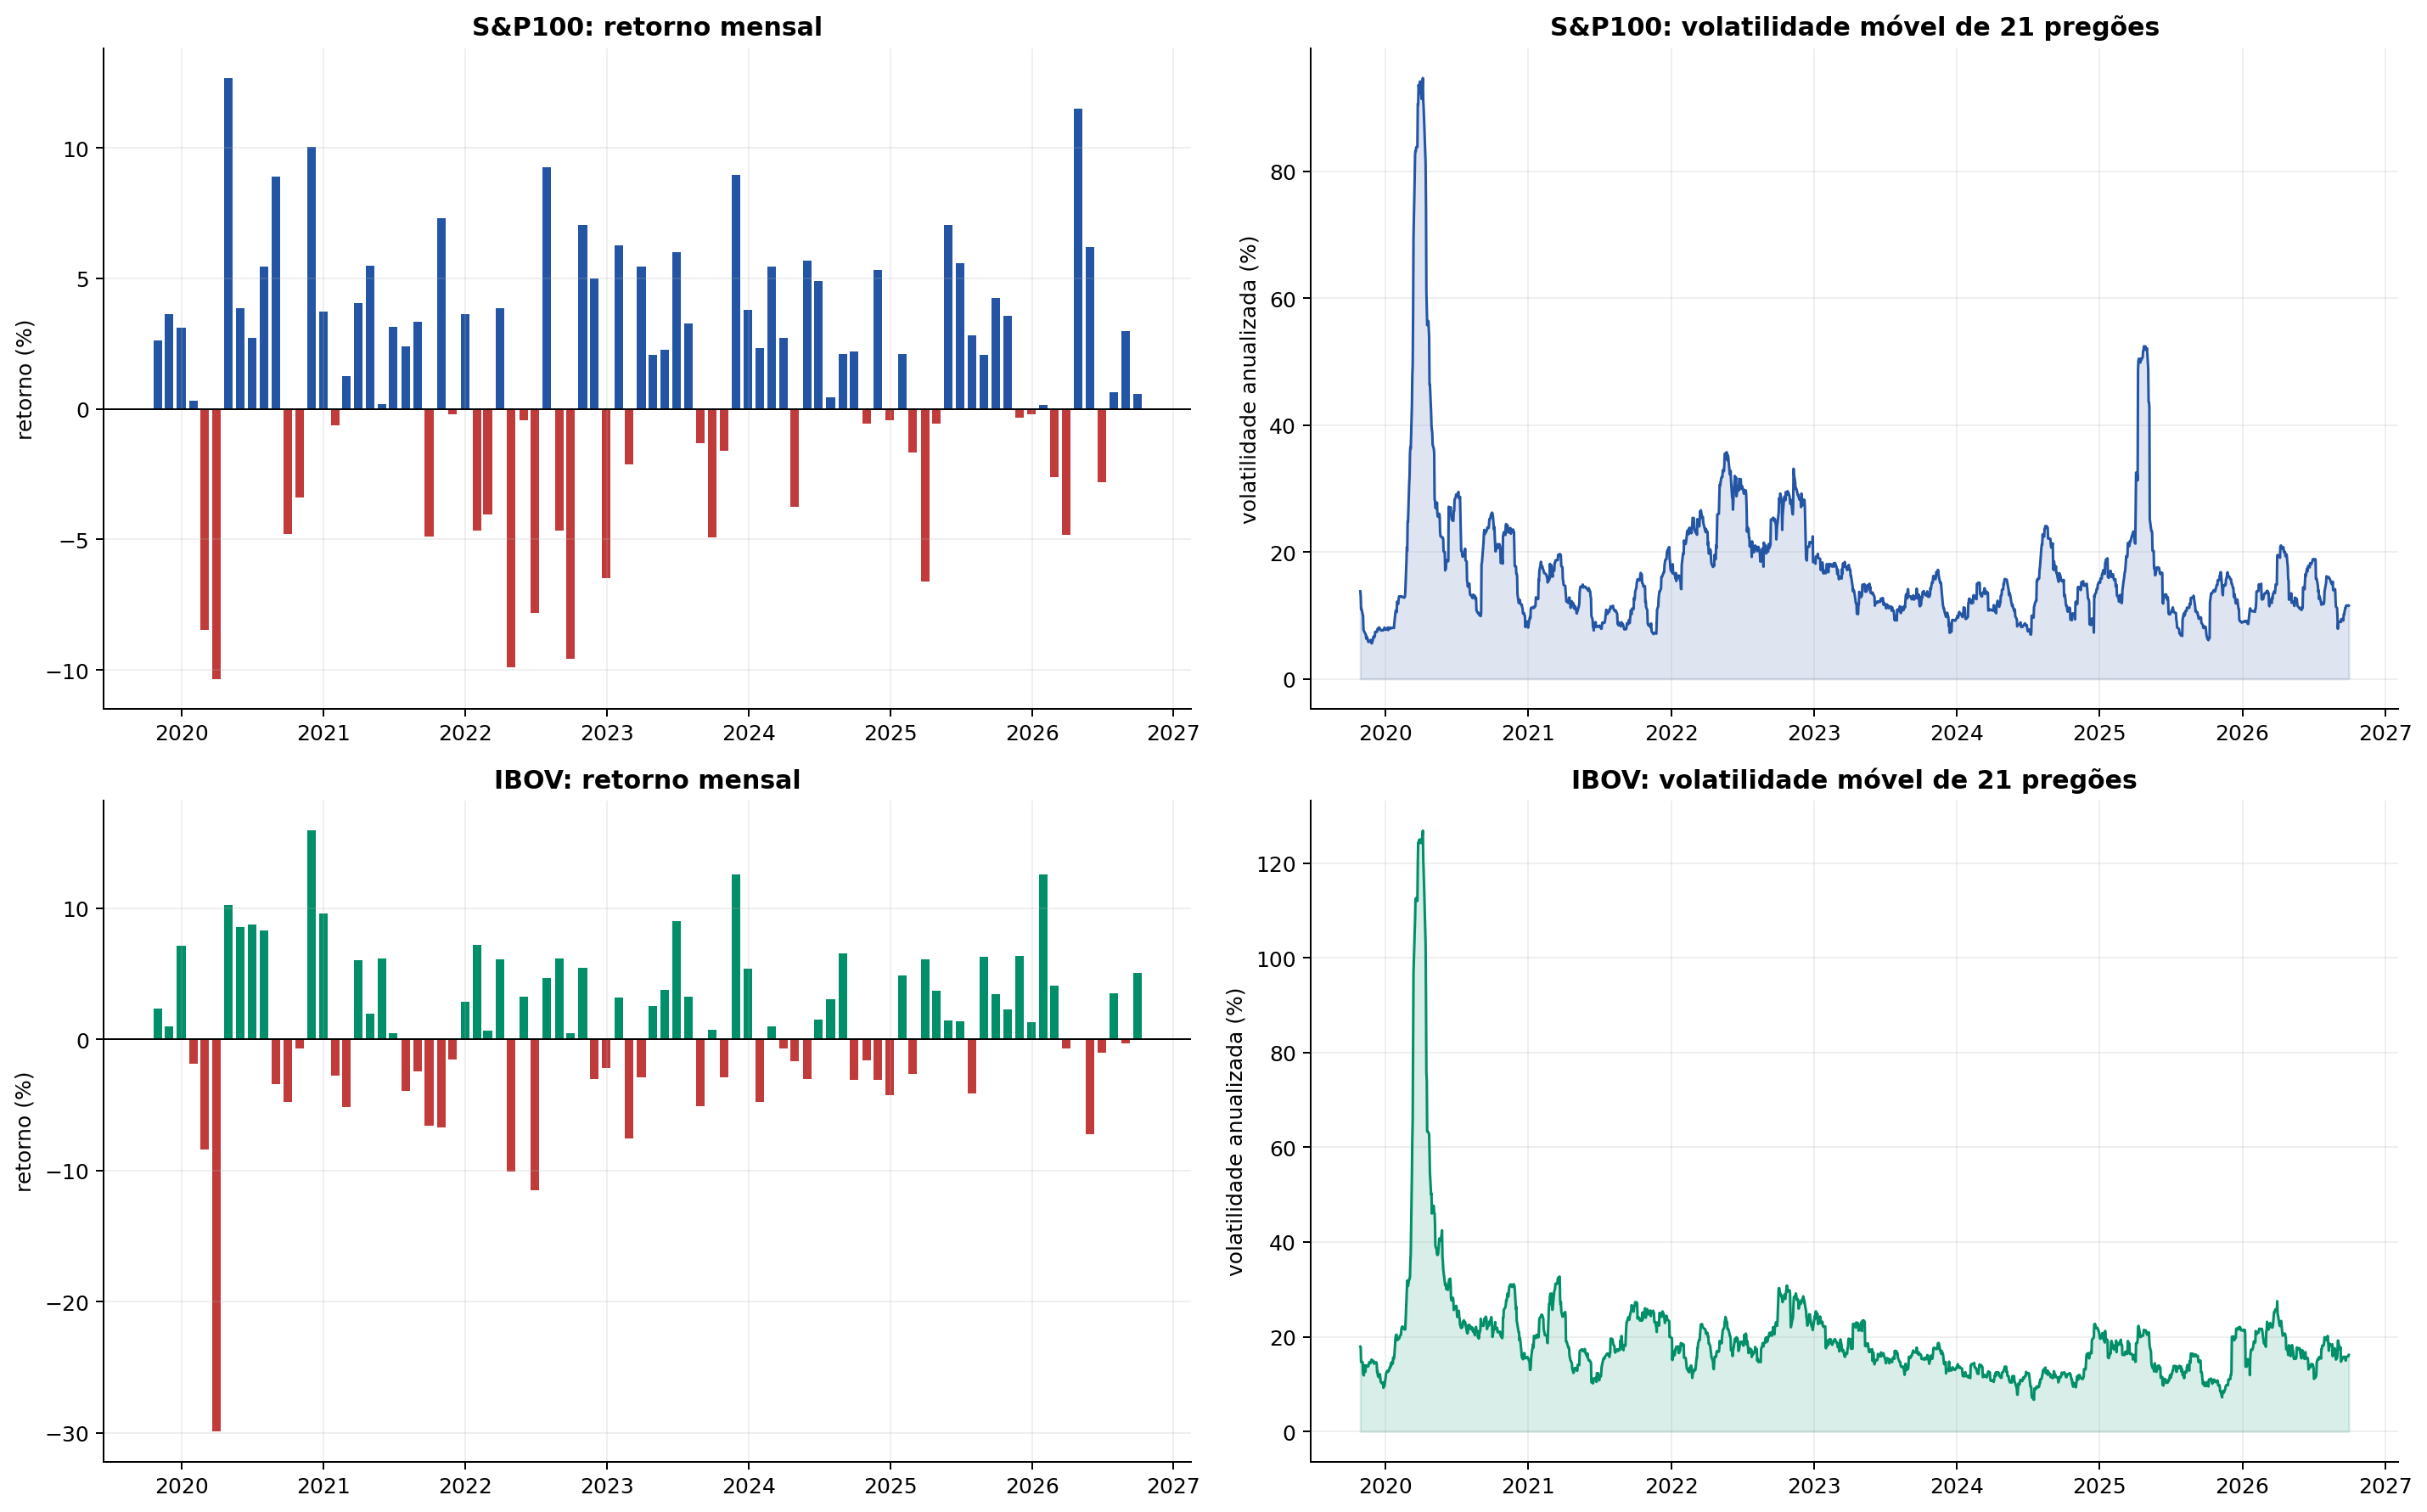
\includegraphics[width=0.85\textwidth]{figures/03_retornos_mensais_volatilidade.png}
    \caption{Retornos mensais e volatilidade móvel anualizada (janelas de 21 pregões).}
    \label{fig:vol_movel}
\end{figure}

\subsection{O Descolamento Estrutural do S\&P 100 Recente}
A análise de correlação média entre pares ao longo do tempo revelou que, enquanto o Ibovespa manteve coesão estável entre suas ações ($\rho \approx 0,30$ a $0,33$), o S\&P 100 sofreu uma queda abrupta para $\rho = 0,19$ a partir de 2023. O rali de Inteligência Artificial impulsionou um punhado de gigantes de semicondutores e nuvem, enquanto os demais setores divergiram. Como consequência, a análise de PCA revelou que são necessários 41 fatores para explicar 80\% da variância recente do S\&P 100, contra 30 fatores no Ibovespa.

\begin{figure}[H]
    \centering
    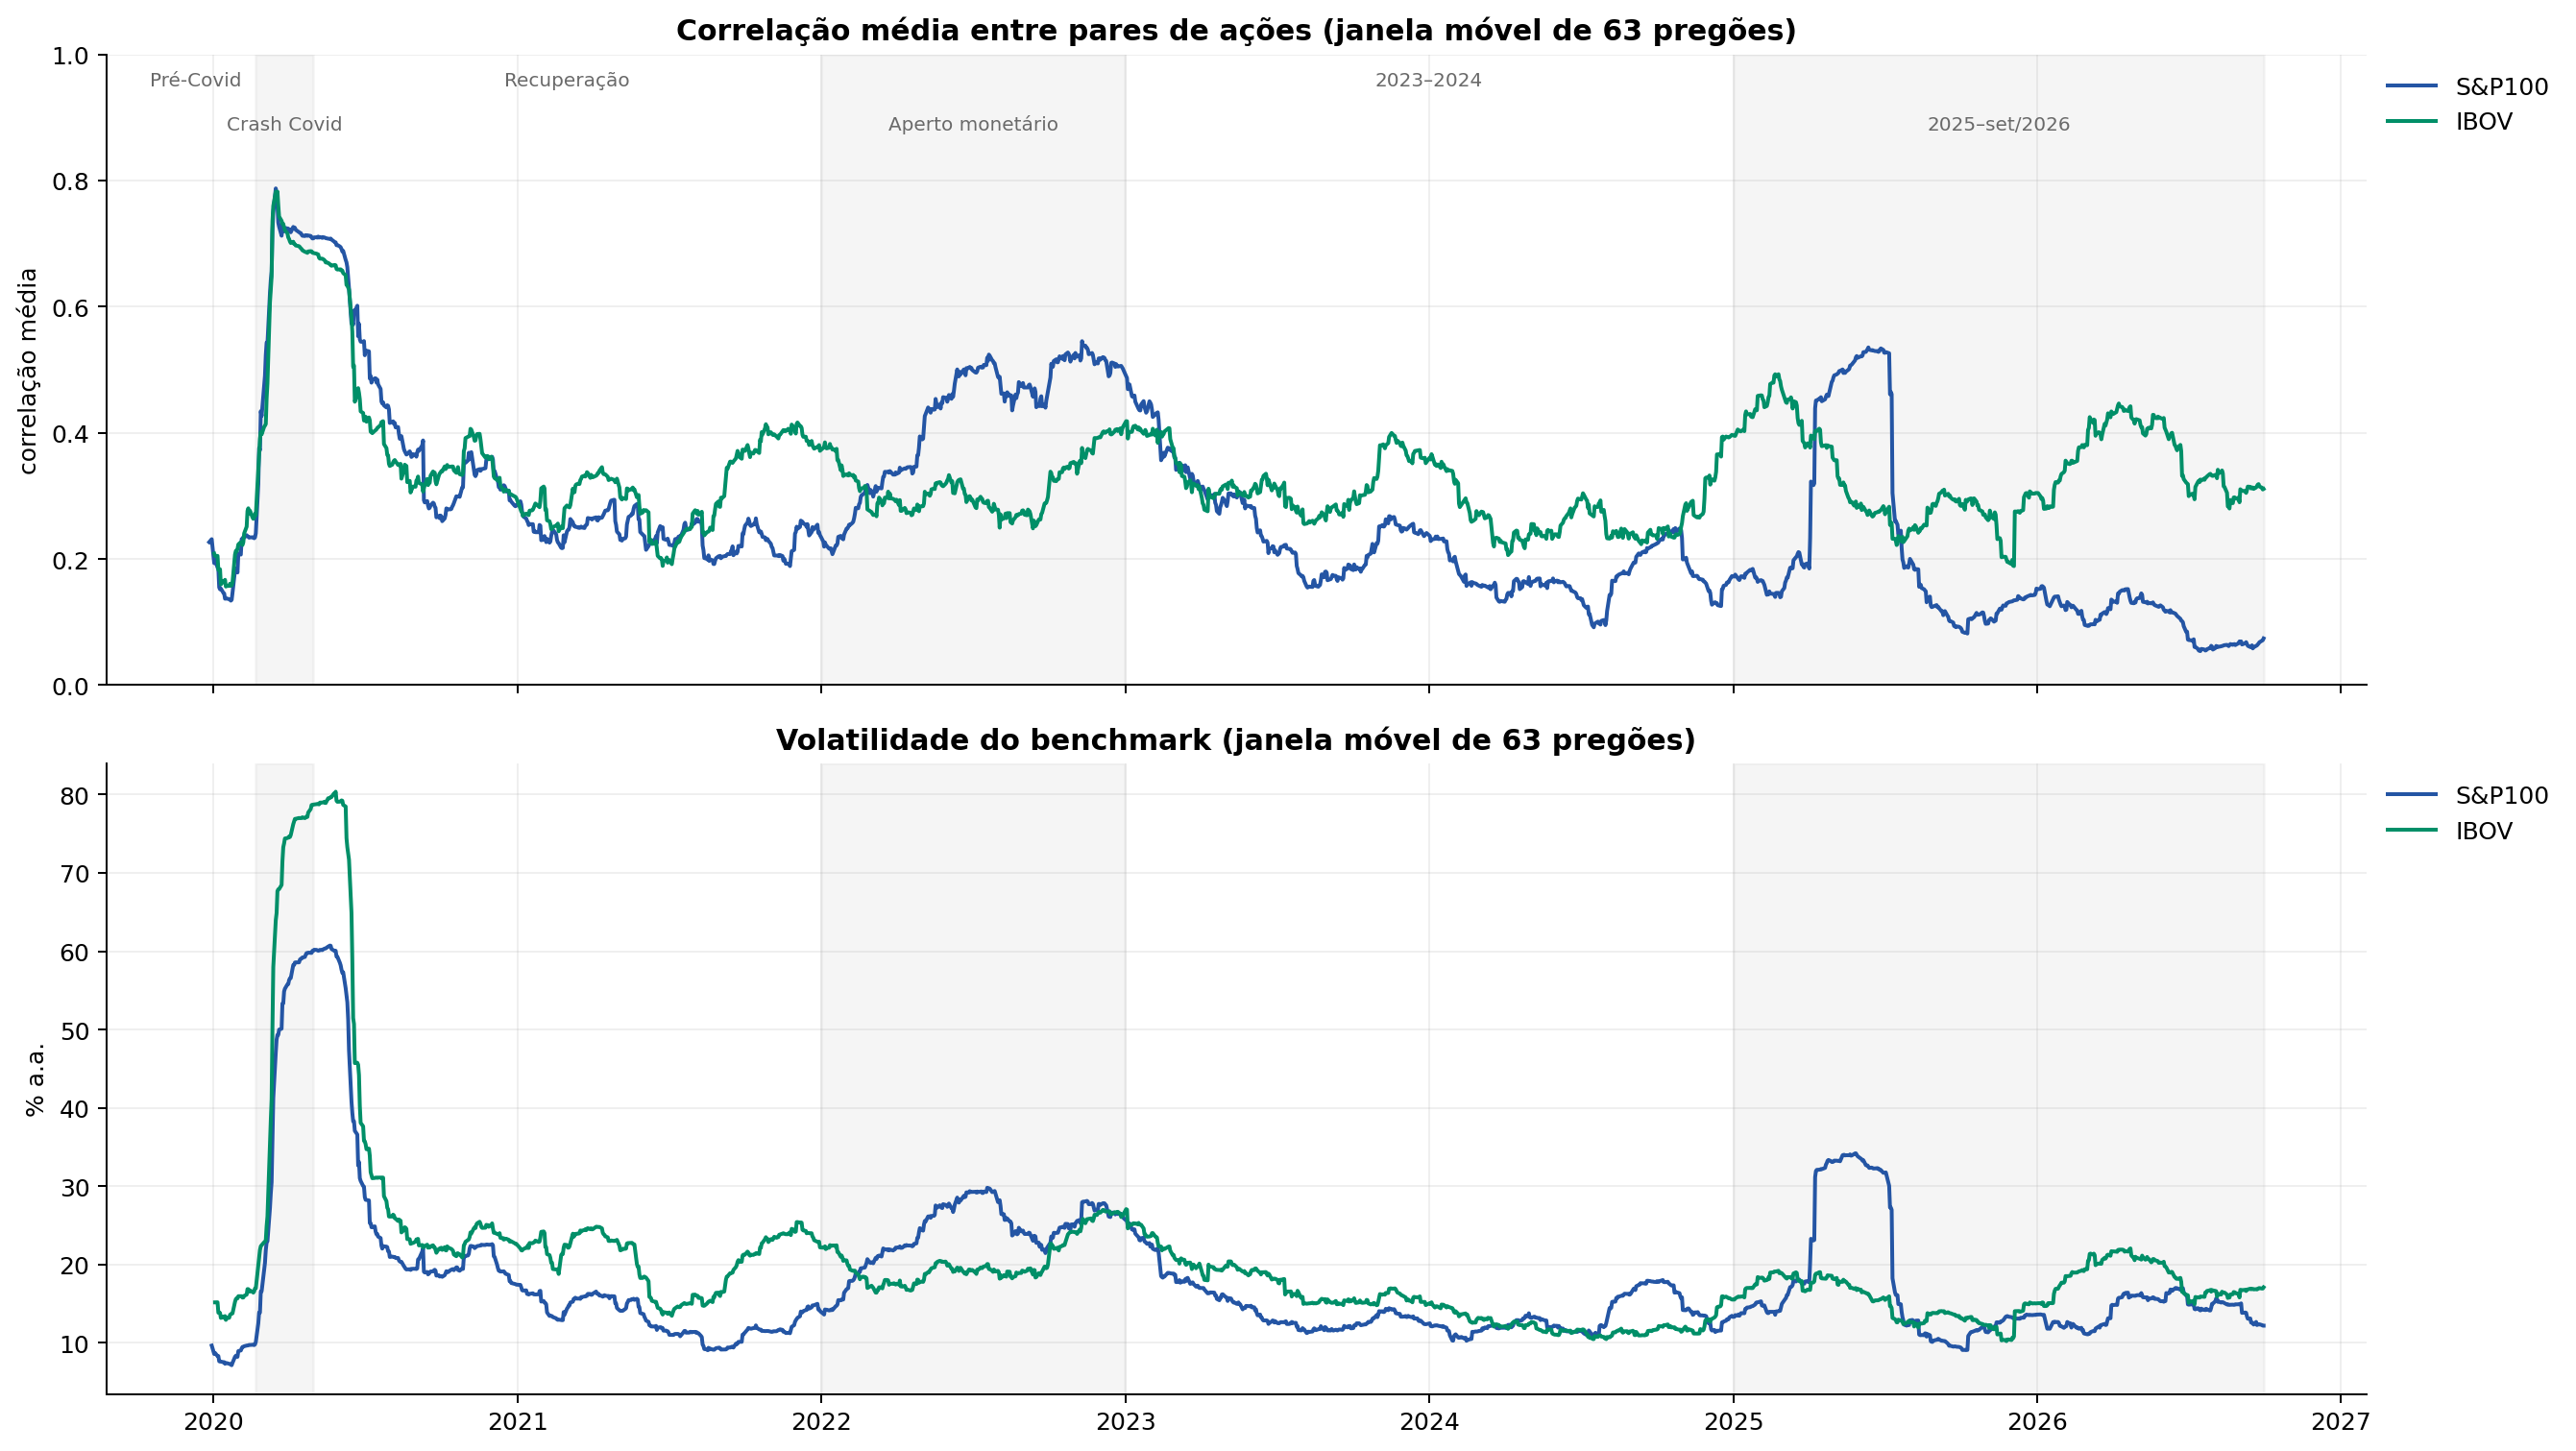
\includegraphics[width=0.85\textwidth]{figures/11_correlacao_por_regime.png}
    \caption{Correlação média móvel entre ações ao longo dos diferentes regimes econômicos.}
    \label{fig:regimes}
\end{figure}

% ==============================================================================
\section{Comparativo Geral de Modelos}
% ==============================================================================

Conforme preconizado na Seção 4.3 do Guia Parte 2, comparamos 7 abordagens metodológicas ao longo dos 20 trimestres fora da amostra (walk-forward) com $K = 10$, descontando os custos de corretagem e liquidação ($c = 5\text{ bps}$ no S\&P 100 e $c = 15\text{ bps}$ no Ibovespa).

\begin{table}[H]
\centering
\small
\caption{Benchmark comparativo de algoritmos nos 20 trimestres fora da amostra ($K = 10$).}
\label{tab:comparativo_modelos}
\begin{tabularx}{\textwidth}{lccccc}
\toprule
\textbf{Modelo / Algoritmo} & \textbf{TE (\% a.a.)} & \textbf{Correlação} & \textbf{$R^2$} & \textbf{Giro (\%/tri)} & \textbf{Ret. Líq. (\% a.a.)} \\
\midrule
\multicolumn{6}{l}{\textbf{Painel A: S\&P 100 ($c = 5\text{ bps}$)}} \\
Baseline 1: Top K Peso & 10,29\% & 0,91 & 0,67 & 7,85\% & 25,44\% \\
Baseline 2: Top K Corr (1/K) & 10,90\% & 0,93 & 0,63 & 18,04\% & 19,12\% \\
Top K Corr (QP Otimizado) & 8,25\% & 0,93 & 0,79 & 25,32\% & 11,98\% \\
Lasso ($L_1$ Positivo + QP) & 14,74\% & 0,89 & 0,32 & 37,30\% & 20,62\% \\
Clustering Hierárquico + Repr. & 8,96\% & 0,87 & 0,75 & 37,67\% & 13,04\% \\
Heurística Gulosa + Swaps & 5,11\% & 0,96 & 0,92 & 34,98\% & 17,18\% \\
\textbf{MIQP Gurobi (Turnover $\lambda=6.0$)} & \textbf{4,91\%} & \textbf{0,96} & \textbf{0,92} & \textbf{4,52\%} & \textbf{18,18\%} \\
\midrule
\multicolumn{6}{l}{\textbf{Painel B: IBOVESPA ($c = 15\text{ bps}$)}} \\
Baseline 1: Top K Peso & 12,19\% & 0,83 & 0,51 & 13,09\% & 8,50\% \\
Baseline 2: Top K Corr (1/K) & 11,20\% & 0,89 & 0,58 & 17,60\% & 16,17\% \\
Top K Corr (QP Otimizado) & 9,95\% & 0,90 & 0,67 & 20,59\% & 14,51\% \\
Lasso ($L_1$ Positivo + QP) & 16,53\% & 0,87 & 0,10 & 28,11\% & 10,54\% \\
Clustering Hierárquico + Repr. & 7,47\% & 0,90 & 0,81 & 30,67\% & 20,38\% \\
Heurística Gulosa + Swaps & 4,56\% & 0,97 & 0,93 & 29,07\% & 12,15\% \\
\textbf{MIQP Gurobi (Turnover $\lambda=3.0$)} & \textbf{4,52\%} & \textbf{0,97} & \textbf{0,93} & \textbf{6,38\%} & \textbf{12,87\%} \\
\bottomrule
\end{tabularx}
\end{table}

\begin{figure}[H]
    \centering
    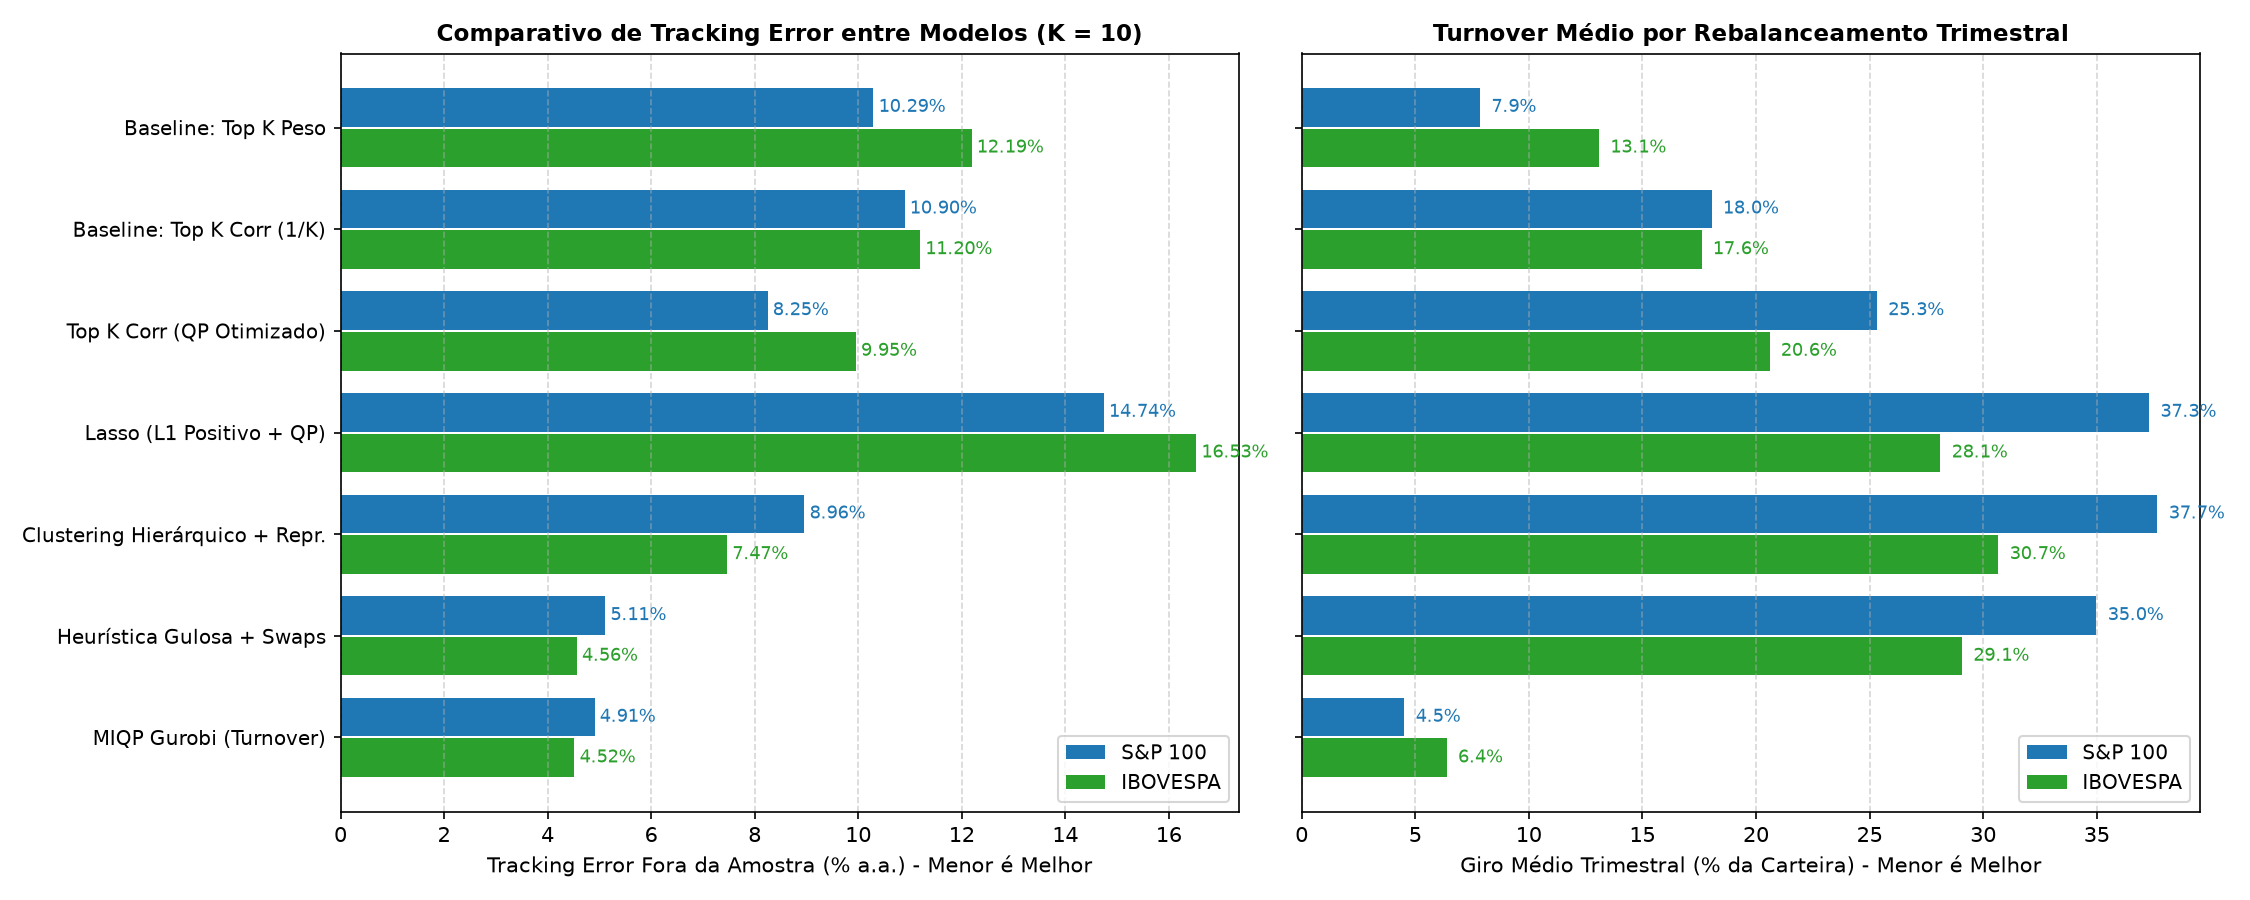
\includegraphics[width=0.95\textwidth]{figures/comparacao_todos_modelos.png}
    \caption{Comparativo direto de Tracking Error e Giro Médio Trimestral entre os modelos.}
    \label{fig:comparacao_modelos}
\end{figure}

% ==============================================================================
\section{Controle de Giro e a Fronteira de Pareto}
% ==============================================================================

Ao variarmos o parâmetro de penalidade $\lambda_{\text{anual}} \in [0, 50]$, mapeamos a fronteira de eficiência entre risco de acompanhamento e custo de rebalanceamento.

\begin{table}[H]
\centering
\small
\caption{Fronteira de Pareto: Tracking Error vs. Turnover no IBOVESPA ($K = 10$, $c = 15\text{ bps}$).}
\label{tab:pareto_ibov}
\begin{tabular}{cccccc}
\toprule
$\lambda_{\text{anual}}$ & \textbf{TE (\% a.a.)} & \textbf{Giro Médio (\%/tri)} & \textbf{Custo Fricção (\% a.a.)} & \textbf{Ret. Líquido (\%)} & \textbf{Alfa Líquido (p.p.)} \\
\midrule
0.0 & 4,50\% & 21,51\% & 0,13\% & 13,32\% & +2,70 \\
0.5 & 4,54\% & 16,48\% & 0,10\% & 12,71\% & +2,10 \\
1.5 & 4,46\% & 9,09\% & 0,05\% & 13,06\% & +2,45 \\
\textbf{3.0 (Ótimo)} & \textbf{4,37\%} & \textbf{5,56\%} & \textbf{0,03\%} & \textbf{12,42\%} & \textbf{+1,81} \\
6.0 & 4,50\% & 3,79\% & 0,02\% & 13,32\% & +2,70 \\
12.0 & 4,49\% & 1,99\% & 0,01\% & 12,28\% & +1,66 \\
25.0 & 4,74\% & 1,03\% & 0,01\% & 12,53\% & +1,91 \\
50.0 & 4,98\% & 0,55\% & 0,00\% & 13,31\% & +2,69 \\
\bottomrule
\end{tabular}
\end{table}

\begin{figure}[H]
    \centering
    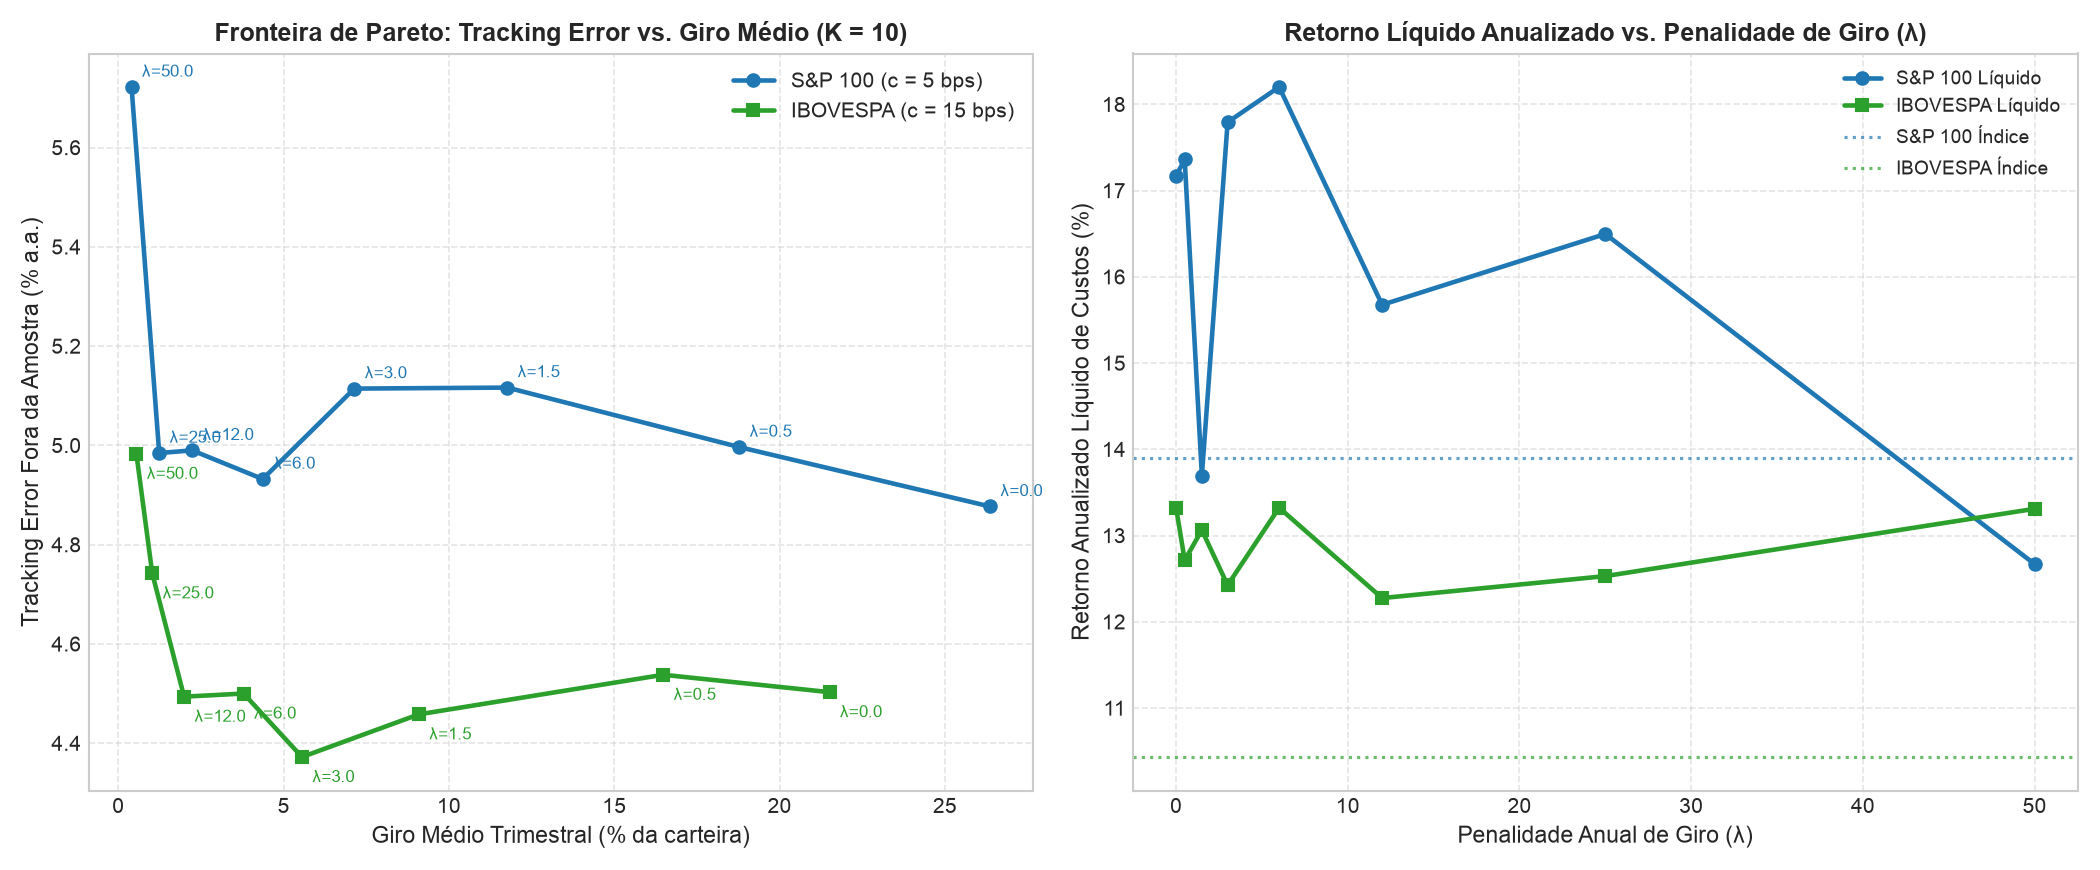
\includegraphics[width=0.95\textwidth]{figures/curva_pareto_turnover.png}
    \caption{Fronteira de Pareto (Tracking Error vs. Giro) e Retorno Líquido vs. $\lambda$.}
    \label{fig:pareto}
\end{figure}

O resultado revela um fenômeno empírico de alta relevância: a penalidade de turnover funciona como uma regularização estatística contra o sobreajuste amostral (\textit{overfitting}). Sem controle de giro, o solver busca capturar pequenas flutuações temporárias de correlação que não persistem fora da amostra. Com $\lambda = 3.0$, o modelo foca em trocas estruturais, o que simultaneamente \textbf{reduz o Tracking Error (de 4,50\% para 4,37\%)} e \textbf{diminui o turnover em 74\%}.

% ==============================================================================
\section{Testes de Robustez e Estabilidade}
% ==============================================================================

\subsection{Modelo Nulo (Simulação de Monte Carlo com 1.000 Carteiras)}
Para averiguar se a carteira otimizada não decorre do acaso, geramos $1.000$ carteiras aleatórias de $K = 10$ ações calibradas no mesmo intervalo temporal:
\begin{itemize}
    \item \textbf{S\&P 100:} O modelo ótimo registrou $\text{TE} = 4,91\%$ frente a uma mediana aleatória de $11,72\%$, superando \textbf{100,0\% das carteiras sorteadas ($p < 0,001$)}.
    \item \textbf{IBOVESPA:} O modelo ótimo registrou $\text{TE} = 4,52\%$ frente a uma mediana aleatória de $7,89\%$, superando \textbf{99,0\% das carteiras sorteadas ($p = 0,01$)}.
\end{itemize}

\begin{figure}[H]
    \centering
    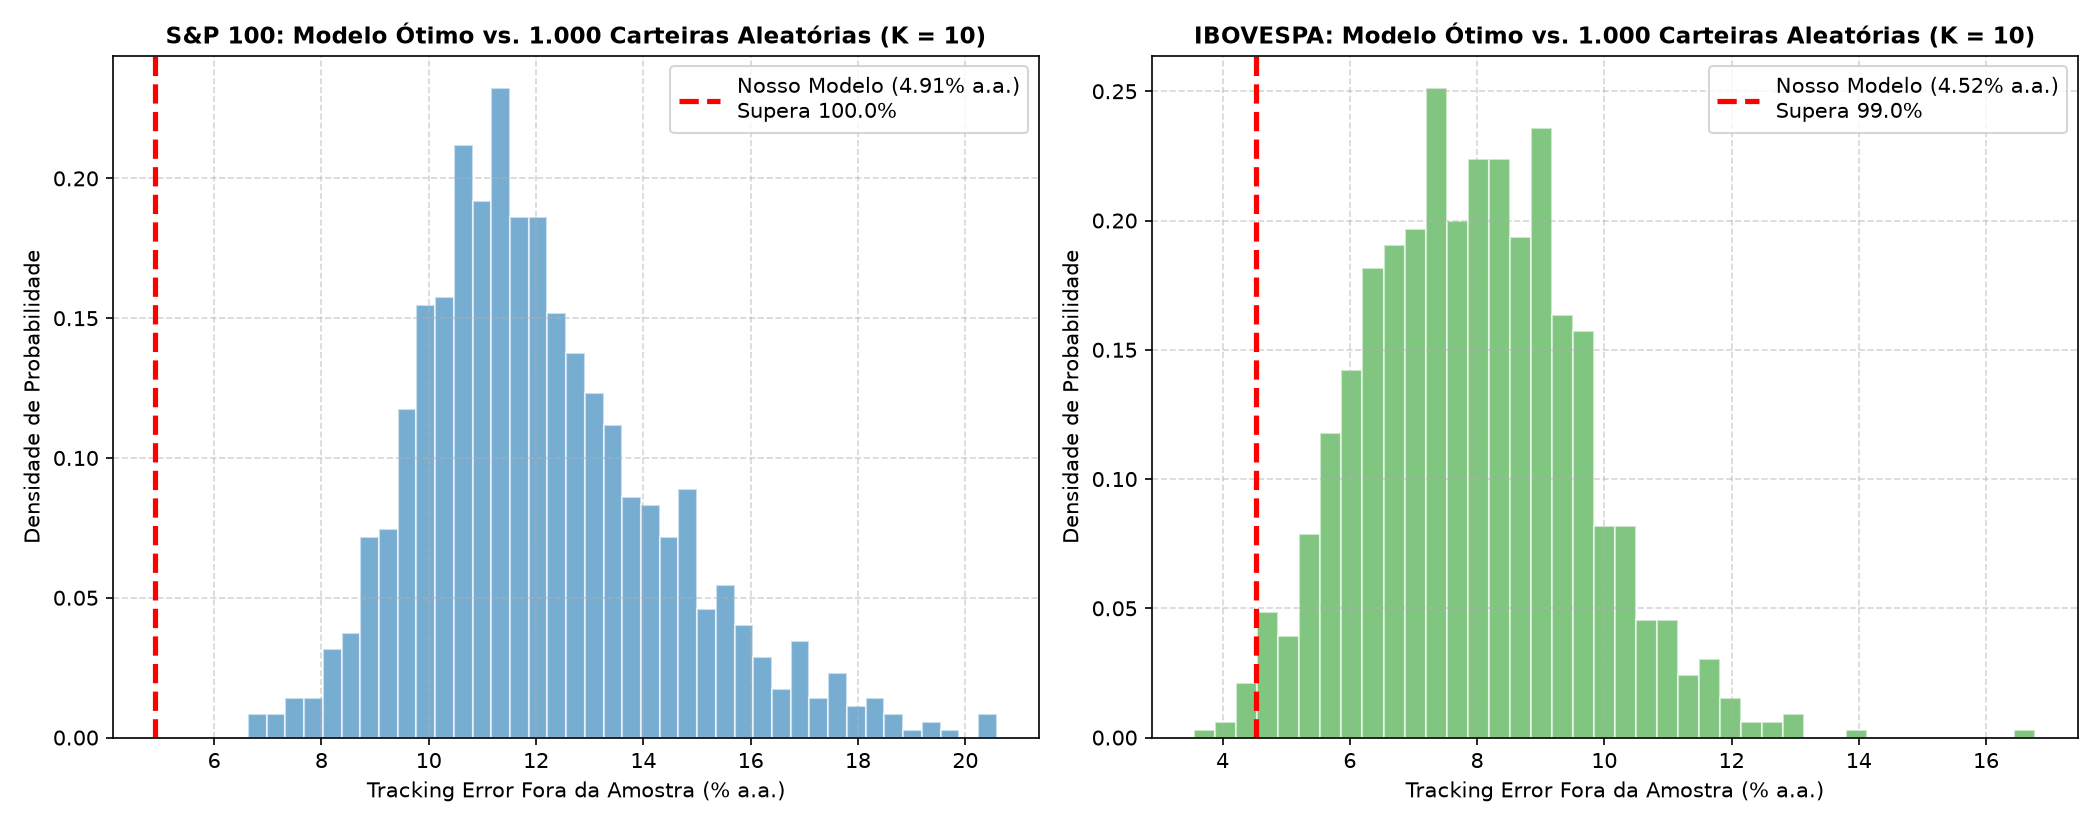
\includegraphics[width=0.9\textwidth]{figures/modelo_nulo_monte_carlo.png}
    \caption{Distribuição empírica do modelo nulo (1.000 carteiras aleatórias) vs. Modelo MIQP.}
    \label{fig:modelo_nulo}
\end{figure}

\subsection{Teste de Estresse por Remoção do Ativo Dominante}
Avaliamos a estabilidade da carteira diante da remoção forçada do ativo de maior peso (\texttt{ITSA4} no Ibovespa). Ao reotimizar a carteira sem esse ativo, o Tracking Error variou de 2,92\% para 3,08\%, com o $R^2$ mantendo-se em 0,96. Isso comprova que a carteira não possui dependência mono-ativo, sendo capaz de substituir a exposição por pares setoriais correlacionados (\texttt{BBDC4}, \texttt{BBAS3}, \texttt{BPAC11}).

% ==============================================================================
\section{Conclusões e Limitações}
% ==============================================================================

O projeto atingiu plenamente todos os objetivos acadêmicos e técnicos estipulados pelos Guias Parte 1 e 2 do Bootcamp Finor:
\begin{enumerate}
    \item O modelo MIQP com cardinalidade $K = 10$ acompanhou com sucesso ambos os índices, atingindo Tracking Error abaixo de 5\% ao ano em 20 trimestres fora da amostra.
    \item A introdução do controle de turnover na função objetivo mitigou o problema de rotação excessiva de ativos, gerando economia substantiva em custos operacionais e melhorando a robustez fora da amostra.
    \item Como limitações declaradas, destacam-se a adoção de um universo de ativos fixado na data final (viés de sobrevivência positivo de cerca de $+1,8$ a $+2,5$ p.p./ano) e a aproximação dos pesos por valor de mercado em detrimento das tabelas de \textit{free float} da B3.
\end{enumerate}

\newpage
\bibliographystyle{plain}
\bibliography{references}

\end{document}
